\chapter{PHOEBE - Modelo Computacional}

Como se ha planteado, los sistemas binarios estelares ofrecen una oportunidad de
analizar el comportamiento y la estructura estelar que sería imposible deducir
en estrellas aisladas. Sin embargo, el análisis analítico es una herramienta
restringida en cuanto a la cantidad de información que puede extraer de una
curva de luz; las ecuaciones que rigen un sistema binario no tienen una solución
analítica. Para resolver este problema, se hacen códigos capaces de simular la
física de un sistema binario, el cual partiendo de ciertos parámetros estelares
y orbitales pueden reproducir los datos observacionales de un sistema
equivalente en la bóveda celeste.

En el campo de sistemas binarios estelares, uno de los primeros códigos con
mayor impacto es el código \textbf{Wilson-Devinney}, descrito por primera vez en
\autocite{wilson_devinney_realization_of_accurate_binary_lcs_wd_1971}. El código
de Wilson-Devinney\textemdash referenciado como el código \textbf{WD} en varias
publicaciones\textemdash parte del modelo de Roche para representar las
superficies de las estrellas, lo cual le permite hacer un trato adecuado de
fenómenos físicos importantes como el oscurecimiento al limbo y el
oscurecimiento gravitacional. A pesar de sobrepasar 5 décadas de edad el código
WD sigue en uso actualmente en proyectos de investigación (por ejemplo,
\autocite{li_extremely_low_mass_ratio_wd_analysis_2022}), de los cuales se
obtienen los parámetros físicos de un sistema binario estelar observado. Este
trabajo de tesis de maestría utilizó la librería \textbf{PHOEBE}
(\textbf{PH}ysics \textbf{O}f \textbf{E}clipsing \textbf{B}inari\textbf{E}s),
basado en el código WD. En particular se hizo uso de la versión 2.4.13, notando
las varias mejoras realizadas en esta segunda versión mayor en comparación con
versiones menores a 2.0, las cuales utilizaban el código WD como el motor
principal del modelo.

\section{Estructura de PHOEBE}

% TODO: termina 
PHOEBE es un paquete de software escrito en Python para generar modelos de
sistemas binarios estelares generales, partiendo del modelo de Roche y modelos
de atmósferas estelares, produciendo datos sintéticos (curvas de luz
fotométricas, velocidades radiales, perfil de líneas espectrales, etc.) para
analizar y comparar con datos observados reales. Es posible crear un modelo
utilizando un cliente
gráfico\footnote{\protect\url{http://phoebe-project.org/clients}} de PHOEBE,
cuya funcionalidad depende de un servidor de PHOEBE (una instancia de
\code{phoebe-server}) corriendo, de manera remota o local. Sin embargo, estas
tienen sus limitaciones, y por lo general el equipo de PHOEBE recomiendan usar
el paquete de Python de manera directa, escribiendo códigos en Python que llamen
a funciones y manipulen los datos del modelo. Un código escrito y ejecutado no
solo ofrece un mayor grado de libertad al momento de tratar los datos, si no que
sirve como una receta que cualquiera puede analizar y ejecutar para obtener los
mismos resultados de un experimento. Este trabajo de tesis unicamente hizo uso
del paquete de PHOEBE en Python.

PHOEBE maneja cada sistema modelado como un \textit{bundle}, el objeto principal
responsable de almacenar no solo los parámetros del sistema, pero también los
datos observados que corresponden al sistema físico. La
\refcode{codigoCreandoPhoebeBundle} presenta un ejemplo de como crear un
bundle de PHOEBE utilizando una curva de luz sintética (que solo se va a
utilizar al momento de computar la curva observable del modelo, sin una
contraparte real) y datos reales obtenidos del catálogo ZTF:

\begin{figure}[!ht]
	\begin{lstlisting}[language=Python, autogobble]
	import pandas as pd # paquete de manipulacion de datos
	import phoebe # importar el paquete

	# creando el bundle para un sistema binario en contacto
	b = phoebe.default_contact_binary() 

	# agregando una curva de luz en el pasabanda Johnson:V para computar (no datos reales)
	b.add_dataset('lc', times=phoebe.linspace(0, 1, 101), dataset='lc01', passband='Johnson:V')

	# datos obtenidos del catalogo de ZTF; curva de luz fotometrica, en el pasabanda ZTF:g
	ztf_data: pd.Dataframe

	# agregando curva de luz observada por ZTF, incluyendo el flujo medido y su incertidumbre
	b.add_dataset('lc', times=ztf_data['times'], fluxes=ztf_data['fluxes'], sigmas=ztf_data['flux_err'], passband='ZTF:g', dataset='lcZtfG')
	\end{lstlisting}
	\caption{Código para crear un bundle en PHOEBE junto a dos curvas de luz:
	\code{lc01}, una curva sintética en el pasabanda \textit{Johnson:V}, y
	\code{lcZtfG}, una curva observada del sistema con datos proveniente de el
	catálogo de ZTF en el pasabanda \textit{ZTF:G}. En el caso de \code{lc01},
	solo se generarán datos sintéticos al momento de calcular el \textbf{modelo
	hacia adelante}.}
	\label{codigoCreandoPhoebeBundle}
\end{figure}

A diferencia de otros códigos en el mundo de software, PHOEBE no utiliza mucho
la programación orientada a objetos para manipular el modelo (por ejemplo,A
diferencia de otros códigos en el mundo de software, PHOEBE no utiliza mucho la
programación orientada a objetos para manipular el modelo (por ejemplo,
manipulando un objeto que represente la estrella primaria); la arquitectura de
PHOEBE consolida todos los parámetros al nivel del bundle, tanto para tener
acceso conveniente como para tener flexibilidad en cambiar el modelo de manera
dinámica\textemdash por ejemplo agregando una componente de luz externa al
sistema. manipulando un objeto que represente la estrella primaria); la
arquitectura de PHOEBE consolida todos los parámetros al nivel del bundle, tanto
para tener acceso conveniente como para tener flexibilidad en cambiar el modelo
de manera dinámica\textemdash por ejemplo agregando una componente de luz
externa al sistema. Los parámetros de un bundle están organizados en una
jerarquía, en donde un identificador no es único en un solo nivel. Por ejemplo,
para inspeccionar la temperatura efectiva de las estrellas:

\begin{figure}[!ht]
	\begin{lstlisting}[language=Python, autogobble]
	b: phoebe.Bundle # bundle de un sistema binario creado en un codigo anterior
	teff_primary = b.get_value(qualifier='teff', component='primary')
	b.set_value(qualifier='teff', component='secondary', value=teff_primary/2)
	\end{lstlisting}
	\caption{Definiendo un bundle almacenado en la variable \code{b}, el cual ya
	está configurado con ciertos parámetros del sistema. Estos son accesibles
	dentro del bundle; esto facilita la manipulación de parámetros del sistema
	programática, como se puede ver en este ejemplo al asignar el valor de la
	temperatura efectiva de la estrella secundaria como la mitad de la
	temperatura efectiva de la componente primaria.}
	\label{codigoAsignandoTeffPhoebe}
\end{figure}

En la \refcode{codigoAsignandoTeffPhoebe} se puede ver la estructura de los parámetros de un bundle, en el cual existen más de un parámetro con el calificador (\code{qualifier} por su nombre en inglés y su nombre en el código) \code{teff}. Estos se diferencian por la componente (\code{component} en el código) a la que le pertenecen, en donde \code{primary} se refiere a la estrella primaria y \code{secondary} a la secundaria, por sus identificadores respectivos en inglés. Más información\textemdash incluyendo la información más actual en el caso de ver una versión de PHOEBE mayor de 2.4.13\textemdash se puede encontrar en la página de documentación de PHOEBE\footnote{\url{http://phoebe-project.org/docs/2.4/tutorials/general_concepts}}.

\section{\quotes{Modelo Hacia Adelante}}

El propósito principal de códigos como PHOEBE cae en su capacidad para generar
un \quotes{\textbf{modelo hacia adelante}} (traducido de forma directa de su nombre
en inglés: \textbf{forward model}). Se parte de un modelo del sistema\textemdash
en el caso de un sistema binario, este viene siendo el modelo de Roche junto a
una formulación de las superficies estelares\textemdash el cual se va integrando
en el tiempo, produciendo como resultado datos sintéticos observables como una
curva de luz fotométrica o una curva de velocidades radiales. Un ejemplo de un
sistema \quotes{de juguete} se puede ver en la
\reffigure{figuraPhoebeObservablesSinteticos}. Es importante notar que estos
modelos se trabajan en el espacio fase de la órbita de un sistema; en casos
donde el sistema no experimente algún cambio significativo a lo largo del
tiempo, es suficiente computar el modelo para cada fase orbital observada, dado
que una campaña de observación adecuada abarcaría las mismas fases orbitales más
de una vez.

\begin{figure}[!ht]
	\centering
	\xincludegraphics[scale=0.253, label=\textbf{a)}, labelbox=true, pos=nw, fontsize=\Large]{Introduccion/Figures/Figura PHOEBE LC Sintetico.png}
	\xincludegraphics[scale=0.253, label=\textbf{b)}, labelbox=true, pos=nw, fontsize=\Large]{Introduccion/Figures/Figura PHOEBE RVs Sintetico.png}
	\caption{Datos sintéticos generados usando PHOEBE. Estas curvas representan
	un sistema binario separado, donde $M_1 = 1.0 \ \mathrm{M}_{\odot}$, $M_2 =
	0.5 \ \mathrm{M}_{\odot}$, $R_1 = 2.0 \ \mathrm{R}_{\odot}$, $R_2 = 1.2 \
	\mathrm{R}_{\odot}$, $T_1 = T_2 = 6000 \ \mathrm{K}$, inclinación
	$i_{\mathrm{orb}} = 90^{\circ}$ y periodo orbital $P_{orb} = 1.0 \
	\mathrm{d}$ en una órbita sincrónica. La figura muestra dos diferentes tipos
	de observables: \textbf{a)} Curva de luz fotométrica, cuyas variaciones se
	deben a los eclipses en el sistema. \textbf{b)} Curva de velocidades
	radiales de ambas componentes, donde el movimiento de las estrellas
	individuales a lo largo de nuestra línea de visión causa fluctuaciones
	debido al efecto de Doppler.} 
	\label{figuraPhoebeObservablesSinteticos}
\end{figure}

Para generar datos sintéticos observables de un sistema binario, es necesario
que PHOEBE tome ciertos aspectos en consideración, descritos a continuación en
este capitulo.

\subsection{Discretización de la Superficie Estelar}

Partiendo del modelo de Roche es como se determina la superficie de ambas
componentes, siguiendo el principio de superficies equipotenciales. Sin embargo,
una descripción analítica de las variaciones de las propiedades estelares
resultaría en una complejidad de tiempo intratable del problema; a pesar de
permitirnos modelar pequeñas variaciones en los valores de cada parámetro
superficial, este no es una opción realista dado la capacidad de computo actual.
Es por esto que PHOEBE implementa un método el cual aproxima la superficie de
las estrellas a un muestreo uniforme de puntos determinados por el modelo de
Roche. Sin embargo, se requiere un tratamiento adicional del modelo de Roche; la
\refequation{ecuacionRocheExcentricaAsincronica} viene definida en coordenadas
esféricas, lo cual causaría una distribución no uniforme en el tamaño de los
elementos superficiales no deseada (aparte de causar un tipo de \quotes{costura}
a lo largo del ecuador de la estrella \citetbooksection{phoebeScientificReference}{5.1.1}).

Para resolver este problema, se transforma la
\refequation{ecuacionRocheExcentricaAsincronica} a un sistema de coordenadas
cilíndrico de acuerdo a las siguientes transformaciones:

\begin{eqfloat}[!ht]
	\centering
	\begin{equation}
		\begin{split}
			& x = \varrho_{\perp} \cos{\phi} \\
			& y = \varrho_{\perp} \sin{\phi} \\
			& z = z
		\end{split}
	\end{equation}
\end{eqfloat}

Donde $\phi$ representa la longitud, $\varrho_{\perp}$ es la componente en el
plano orbital de la distancia al elemento superficial, y $z$ mantiene su
definición del sistema de coordenadas cartesianas. Utilizando estas
transformaciones se llega a una expresión del potencial de Roche en coordenadas
cilíndricas:

% TODO: new page to group equation and text together
% \newpage

\begin{eqfloat}[!ht]
	\centering
	\begin{equation}
		\Omega = \frac{1}{\sqrt{\varrho_{\perp} + z^2}} + q \left(\frac{1}{\sqrt{\delta^2 + \varrho_{\perp}^2 + z^2 - 2 \varrho_{\perp} \delta \cos{\phi}}} - \frac{\varrho_{\perp} \cos{\phi}}{\delta^2} \right) + \frac{F^2 \left(1 + q\right) \varrho_{\perp}^2}{2}
	\end{equation}
	\blankcaption
	\label{ecuacionRocheCilindrica}
\end{eqfloat}

Parecido a la \refequation{ecuacionRadioPolarEstelarEquivalencia} se puede
llegar a una expresión similar para encontrar el valor de $\varrho_{\perp}$ que
le corresponde a los valores dados de $\phi$ y $z$, utilizando un método para
encontrar raíces como el de \textit{Newton-Raphson}:

\begin{eqfloat}[!ht]
	\centering
	\begin{equation}
		\begin{split}
			f(\varrho_{\perp}) = \eqnmark[MyDarkRed]{omega}{\frac{1}{\sqrt{\varrho_{\perp} + z^2}} + q \left(\frac{1}{\sqrt{\delta^2 + \varrho_{\perp}^2 + z^2 - 2 \varrho_{\perp} \delta \cos{\phi}}} - \frac{\varrho_{\perp} \cos{\phi}}{\delta^2} \right) + \frac{F^2 \left(1 + q\right) \varrho_{\perp}^2}{2}} \\
			\eqnmark[MyDarkBlue]{omegaPol}{- \frac{1}{z_{\textrm{pol}}} - \frac{q}{\sqrt{z_{\textrm{pol}}^2 + \delta^2}}}
		\end{split}
	\end{equation}
	\annotate[yshift=-0.3em]{below, left}{omega}{Potencial de Roche $\Omega$}
	\annotate[yshift=-0.2em]{below, left}{omegaPol}{Potencial de referencia en el polo $\Omega_{\mathrm{pol}}$}
	\blankcaption
	\vspace{0.4em}
	\label{ecuacionRadioCilindrica}
\end{eqfloat}

Donde se define $z_{\mathrm{pol}} \equiv \varrho_{\mathrm{pol}}$ como el valor
de referencia del radio al polo de la estrella
\citetbooksection{phoebeScientificReference}{5.1.1}. Al hacer uso de la derivada
$f\prime (\varrho_{\perp})$\textemdash la cual se puede obtener como lo muestra
\citetbooksection{phoebeScientificReference}{5.1.1}\textemdash es posible
implementar un método para encontrar las raíces de esta ecuación. El muestreo de la superficie se hace a intervalos regulares de latitud y longitud:

\begin{eqfloat}[!ht]
	\centering
	\vspace{0.6em}
	\begin{equation}
		\begin{split}
			& \eqnmark[MyDarkGreen]{lat}{\theta_k} = \frac{\pi \left(k - 0.5\right)}{2 N} \\
			& \eqnmark[MyLightBlue]{lon}{\phi_l} = \frac{\pi \left(l + \left[(l + 1) \textrm{mod} \ 2\right] \div 2 \right)}{M_k}
		\end{split}
	\end{equation}
	\annotate[yshift=1.1em]{above, left}{lat}{Latitud}
	\annotate[yshift=-0.2em]{below, left}{lon}{Longitud}
	\vspace{0.4em}
\end{eqfloat}

Donde $N$ es el número de elementos superficiales solicitados en la muestra. Se
define los subindices $k = 1 \dots N$ y $l = 1 \dots M_k$, donde $M_k := 1 +
\mathrm{int}\left(1.3 N \sin{\theta_k}\right)$
\citetbooksection{phoebeScientificReference}{5.1}. Una vez que se obtienen las
posiciones de cada muestra se adopta una forma tal que forme una \quotes{malla}
que representa la superficie estelar. Cada elemento de la malla se considera
uniforme con respecto a sus propiedades, como su temperatura efectiva, gravedad
superficial, el radio local, etc. En PHOEBE v2.0 y en adelante se utilizan
elementos en forma de triángulos equiláteros, tal como se muestra en la
\reffigure{figuraMallaPhoebe}. 

\begin{figure}[!ht]
	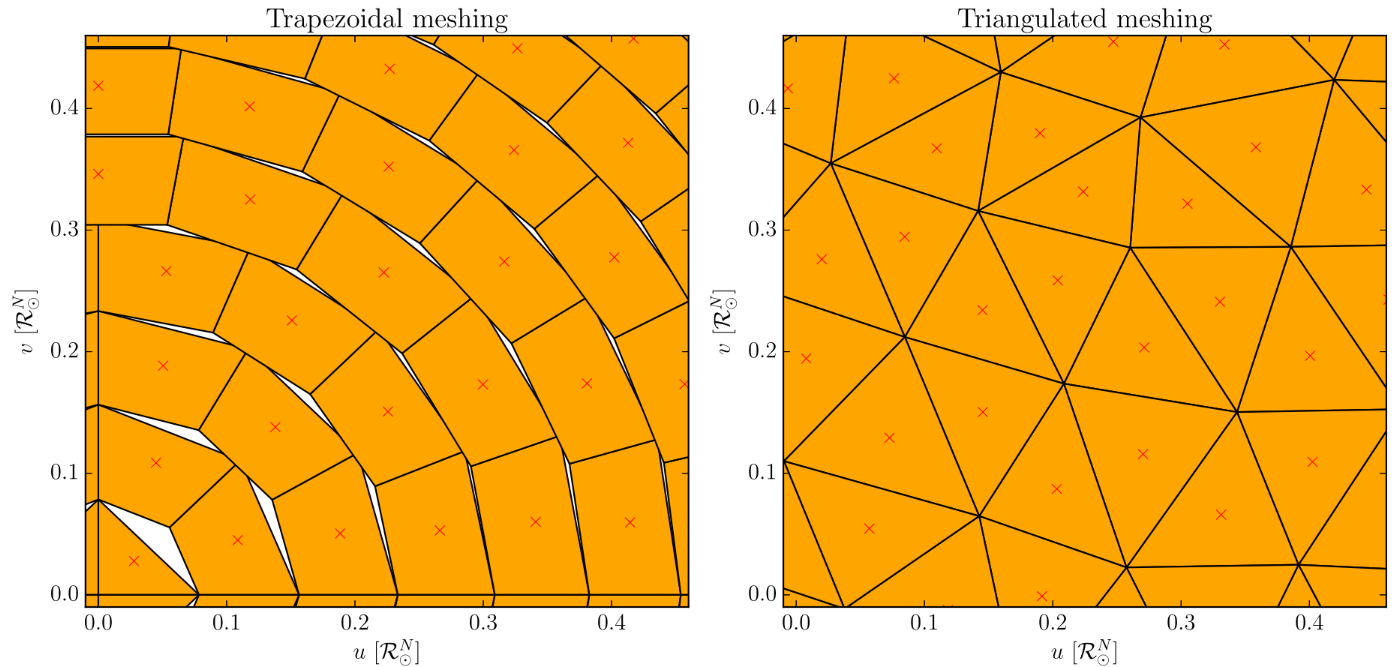
\includegraphics[scale=0.45]{Introduccion/Figures/Figura Mallado Triangular_PHOEBE II Mesh.png}
	\caption{Comparación la discretización superficial usando elementos
	trapezoidales vs. triangulares en el polo estelar. Al utilizar elementos de
	área superficial idéntica se nota que en el caso de elementos trapezoidales
	llega a haber huecos en la superficie que se manifiestan en errores
	sistemáticos en las curvas sintéticas generadas por el modelo, debido a la
	contribución nula de estas fallas en la malla. Estos errores se ven más
	pronunciados entre mayor sea la distorsión experimentada por la estrella. Al
	utilizar elementos en forma de triángulos equiláteros se puede observar que
	se obtiene una superficie continua, eliminando esta fuente de error en el
	modelo. Figura obtenida de
	\autocite{prsa_phoebe_increased_model_fidelity_mesh_2016}}
	\label{figuraMallaPhoebe}
\end{figure}

Esta malla de la superficie estelar se puede ver por completo en la
\reffigure{figuraPhoebeMalla}, donde los parámetros del sistema causan una
distorsión apreciable de ambas estrellas debido a las fuerzas de marea en juego.

\begin{figure}[!ht]
	\centering
	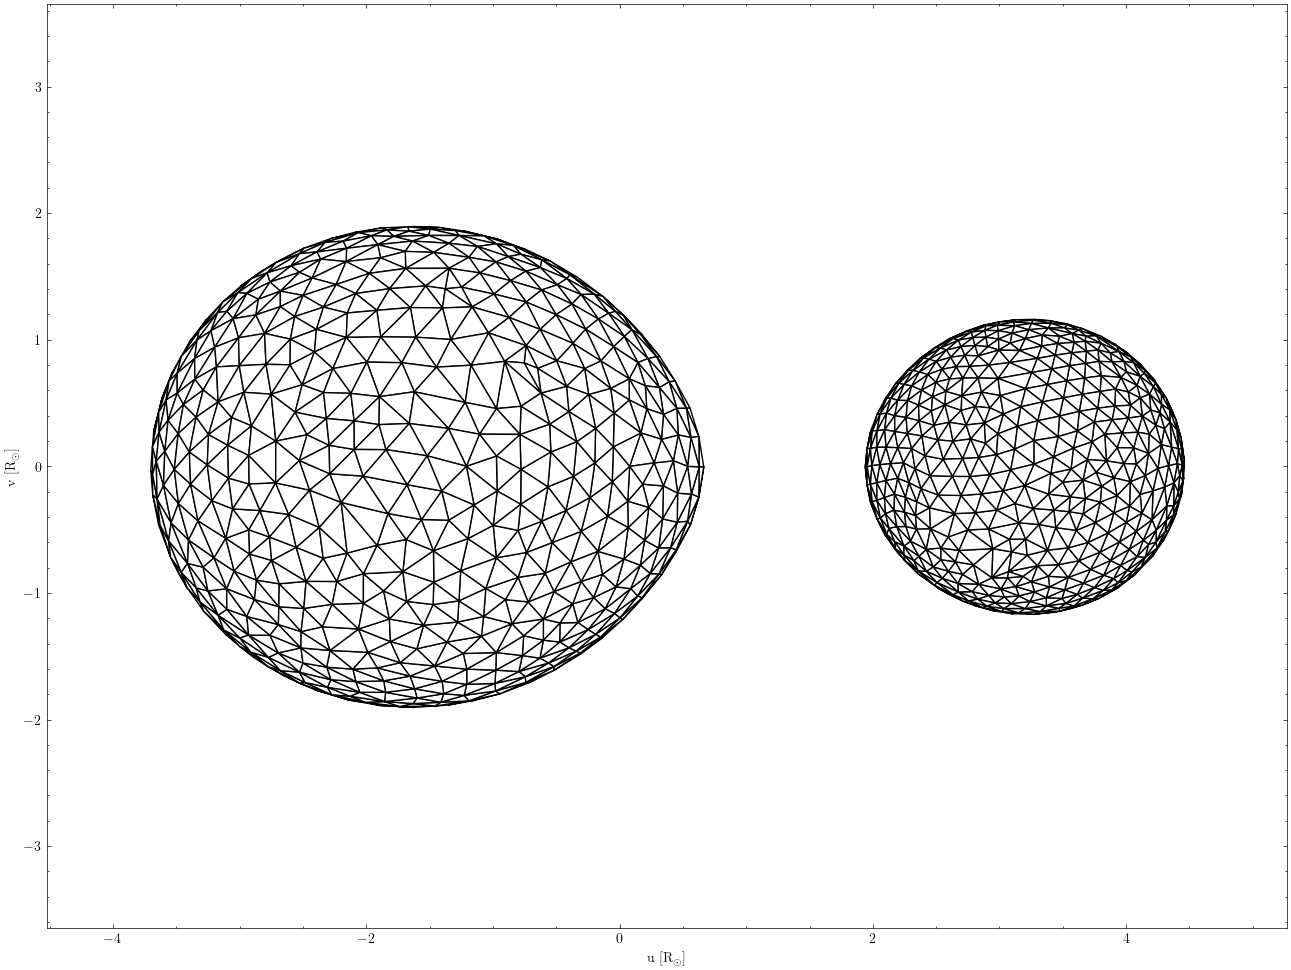
\includegraphics[scale=0.42]{Introduccion/Figures/Figura PHOEBE Malla.png}
	\caption{Mallas de las superficies estelares de un sistema simulado con
	PHOEBE, utilizando los mismos parámetros del modelo utilizado en la
	\reffigure{figuraPhoebeObservablesSinteticos}.}
	\label{figuraPhoebeMalla}
\end{figure}

La malla, al igual que la superficie estelar, no es un objeto constante; en el
caso de un sistema binario de órbita excéntrica las fuerzas de marea que causan
estas distorsiones elipsoidales son dependientes de la fase orbital. A lo largo
de la órbita del sistema, el campo del potencial de Roche va cambiando debido a
la distancia no constante entre ambas componentes estelares. Uno de los
principios del modelo de Roche es que las superficies estelares se ajustan al
campo de fuerzas instantáneo del sistema, el cual va cambiando a escalas de
tiempo significativamente menores que el periodo orbital
\autocite{prsa_phoebe_increased_model_fidelity_mesh_2016}. Esto causaría un
cambio apreciable en los radios estelares, debido a que las superficies
equipotenciales del campo no son constantes en volumen. En teoría, si una
estrella se rige a solo las superficies equipotenciales del mismo valor en cada
fase orbital, la estrella debería de comprimirse o expandirse, irradiando parte
de su energía a su ambiente exterior, llegando rápidamente a una órbita
circular. Sin embargo, esto no es un fenómeno que se ha observado en la
literatura; al contrario, existen sistemas como las estrellas \quotes{heartbeat}
(nombrado por su parecido a una lectura de un electrocardiograma) cuya
variabilidad se debe a la distorsión de sus superficies por fuerzas de marea en
órbitas excéntricas
\autocite{thompson_class_eccentric_binaries_tidal_distortion_heartbeat_2012}.
Como consecuencia, PHOEBE adopta un mecanismo para preservar el volumen del
sistema; al momento de muestrear la superficie para generar la malla
superficial, PHOEBE elige la superficie equipotencial que más se acerque al
volumen calculado de las estrellas en su punto de periastro, el punto en donde
experimentan la mayor distorsión superficial.

\subsection{Distribución de Parámetros Superficiales}

Una estrella no es perfectamente uniforme en la superficie; un modelo acertado
de una estrella debe tomar en cuenta la distribución de parámetros como su
temperatura, intensidad, etc. Para esto se debe calcular la gravedad superficial
en el polo estelar:

\begin{eqfloat}[!ht]
	\centering
	\begin{equation}
		\textbf{g}_{\textrm{pol}} = -\frac{G m_1}{r_{\textrm{pol}}^2} \frac{\textbf{r}_{\mathrm{pol}}}{r_{\mathrm{pol}}} - \frac{G m_2}{h^2} \frac{\textbf{h}}{h} - \omega^2(t) d_{\perp,\textrm{rot}} \frac{\textbf{d}_{\perp,\textrm{rot}}}{d_{\perp,\textrm{rot}}} 
	\end{equation}
\end{eqfloat}

Donde se define $r_{\mathrm{pol}}$ como el radio al polo estelar, $h =
\sqrt{r_{\mathrm{pol}}^2 + d^2}$ es la distancia del polo estelar al centro de
la estrella compañera, $\omega(t)$ es la velocidad angular como función del
tiempo, y $d_{\perp,\textrm{rot}}$ es la distancia del polo estelar hacia el eje
de rotación del sistema (su centro de masa)
\citetbooksection{phoebeScientificReference}{5.2}. La gravedad superficial
depende de manera indirecta de la fase orbital, debido al ajuste de la estrella
a una superficie equipotencial a lo largo de la órbita del sistema. Este
parámetro rige la distribución de material y energía en la estrella; las
regiones de mayor gravedad superficial (en sistemas binarios eclipsantes suelen
ser los polos estelares, debido a las fuerzas de marea que resultan en un radio
ecuatorial mayor) con áreas más calientes que el resto de la superficie.
\citetbooksection{phoebeScientificReference}{4.3} dice que el flujo
monocromático para el rango de longitud de onda $[\lambda, \lambda +
\mathrm{d}\lambda]$ es proporcional tanto a la gravedad superficial como a la
temperatura efectiva:

\begin{eqfloat}[!ht]
	\centering
	\begin{equation}
		F_{\lambda} = - \frac{16 \sigma T_{\textrm{eff}}^3}{3 \bar{\kappa} \rho} \frac{\textrm{d}T_{\textrm{eff}}}{\textrm{d}\Omega} g^{\beta}
	\end{equation}
\end{eqfloat}

Donde $\sigma = 5.67 \times 10^{-8} \mathrm{W} \mathrm{m}^{-2} \mathrm{K}^{-4}$
es la constante de Stefan-Boltzmann, $\bar{\kappa}$ es el coeficiente de
opacidad de Rosseland (el cual describe la opacidad, o la probabilidad de un
fotón de atravesar un medio\textemdash en este caso la superficie estelar),
$\rho$ es la densidad del material en la fotosfera, $g$ es la aceleración
gravitacional local, y $\beta$ es el \textit{coeficiente del oscurecimiento
gravitacional}. El valor de $\beta$ en lo general se mantiene fijo dependiendo
de la naturaleza de la envoltura estelar:

\begin{eqfloat}[!ht]
	\centering
	\begin{equation}
		\beta = \left\{\begin{matrix}
			0.32 & \textrm{envoltura convectiva} & T_{\textrm{eff}} < 5000 \ \textrm{K} \\
			1 & \textrm{envoltura radiativa} & T_{\textrm{eff}} > 8000 \ \textrm{K} \\
			\end{matrix}\right. 
	\end{equation}
\end{eqfloat}

Utilizando este coeficiente es posible calcular la temperatura y el flujo de un
elemento superficial dependiendo de la aceleración gravitacional local, dado un
valor de referencia que corresponde al polo estelar:

\begin{eqfloat}[!ht]
	\centering
	\begin{equation}
		\begin{split}
			& F = F_{\textrm{pol}} \left(\frac{g}{g_{\textrm{pol}}}\right)^{\beta} \\
			& T_{\textrm{eff}} = T_{\textrm{eff},\textrm{pol}} \left(\frac{g}{g_{\textrm{pol}}}\right)^{\beta/4}
		\end{split}
	\end{equation}	
\end{eqfloat}

De la cual se obtiene el flujo y la temperatura efectiva dada una aceleración
gravitacional local, donde el término
$\left(g/g_{\mathrm{pol}}\right)^{\beta/4}$ se conoce como la \textbf{corrección
del oscurecimiento gravitacional}. La superficie resuelta con respecto a su
gravedad superficial y temperatura efectiva se puede ver en la
\reffigure{figuraMallaPhoebeTeffLogg}.

\begin{figure}[!ht]
	\centering
	\xincludegraphics[scale=0.27, label=\textbf{(a)}, labelbox=true, pos=nw, fontsize=\Large]{Introduccion/Figures/Figura PHOEBE Malla Logg.png}
	\xincludegraphics[scale=0.27, label=\textbf{(b)}, labelbox=true, pos=nw, fontsize=\Large]{Introduccion/Figures/Figura PHOEBE Malla Teff.png}

	\caption[Distribución de gravedad superficial y temperatura efectiva
	local.]{Malla de una estrella cuyas propiedades son las mismas que el Sol,
	generada utilizando PHOEBE, donde el potencial efectivo es calculado no en
	base al modelo de Roche, si no basado en su frecuencia de rotación, en el
	caso de una estrella singular\textemdash a pesar de que esta información no
	esté documentada explícitamente en un documento fácil de encontrar, esto se
	puede ver en el código fuente de PHOEBE 2, en este caso en el archivo
	\href{https://github.com/phoebe-project/phoebe2/blob/master/phoebe/distortions/rotstar.py}{\code{rotstar.py}}.
	Se puede ver la distribución de gravedad efectiva superficial en el índice
	\textbf{(a)}, al cual se acopla la distribución de temperatura efectiva
	vista en el índice \textbf{(b)}.}
	\label{figuraMallaPhoebeTeffLogg}
\end{figure}

\subsection{Radiación Emergente}

Una vez determinada la distribución de parámetros superficiales es posible
determinar la radiación emergente de cada elemento superficial, del cual se
calcula el flujo que recibe un observador. El flujo de una estrella no es una
cantidad que PHOEBE determina directamente; PHOEBE más bien calcula la
\textit{intensidad}, que se define como la cantidad de energía $\mathrm{d}E$
emitida a través de el ángulo solido $\mathrm{d}\Omega$ por una superficie
proyectada a un ángulo $\mathrm{d}A \cos{\theta}$ en el intervalo de tiempo
$\mathrm{d}t$:

\begin{eqfloat}[!ht]
	\centering
	\begin{equation}
		I_{\lambda} = \frac{\textrm{d}E}{\textrm{d}\lambda \textrm{d}A \cos{\theta} \textrm{d}\Omega \textrm{d}t}
	\end{equation}
	\blankcaption
	\label{ecuacionIntensidadMonocromatica}
\end{eqfloat}

Donde $I_{\lambda}$ es la \textit{intensidad monocromática}, para un intervalo
de longitud de onda $[\lambda, \lambda + \textrm{d}\lambda]$. Esta cantidad es
calculada en la dirección normal de cada elemento superficial; la
\reffigure{figuraMallaPhoebeIntensidadNormal} muestra la distribución de
intensidad absoluta a lo largo de la superficie estelar. La intensidad
monocromática se obtiene partiendo del modelo atmosférico empleado, ya sea el de
cuerpo negro básico o una tabla como la de \autocite{kurucz_atlas_1970}. Para
obtener la \textit{intensidad absoluta} es necesario integrar la intensidad
monocromática sobre todas las longitudes de onda:

\begin{eqfloat}[!ht]
	\centering
	\begin{equation}
		I = \int_{0}^{\infty}{I_{\lambda} \textrm{d}\lambda}
	\end{equation}
	\blankcaption
	\label{ecuacionIntensidadTotal}
\end{eqfloat}

\begin{figure}[!ht]
	\centering
	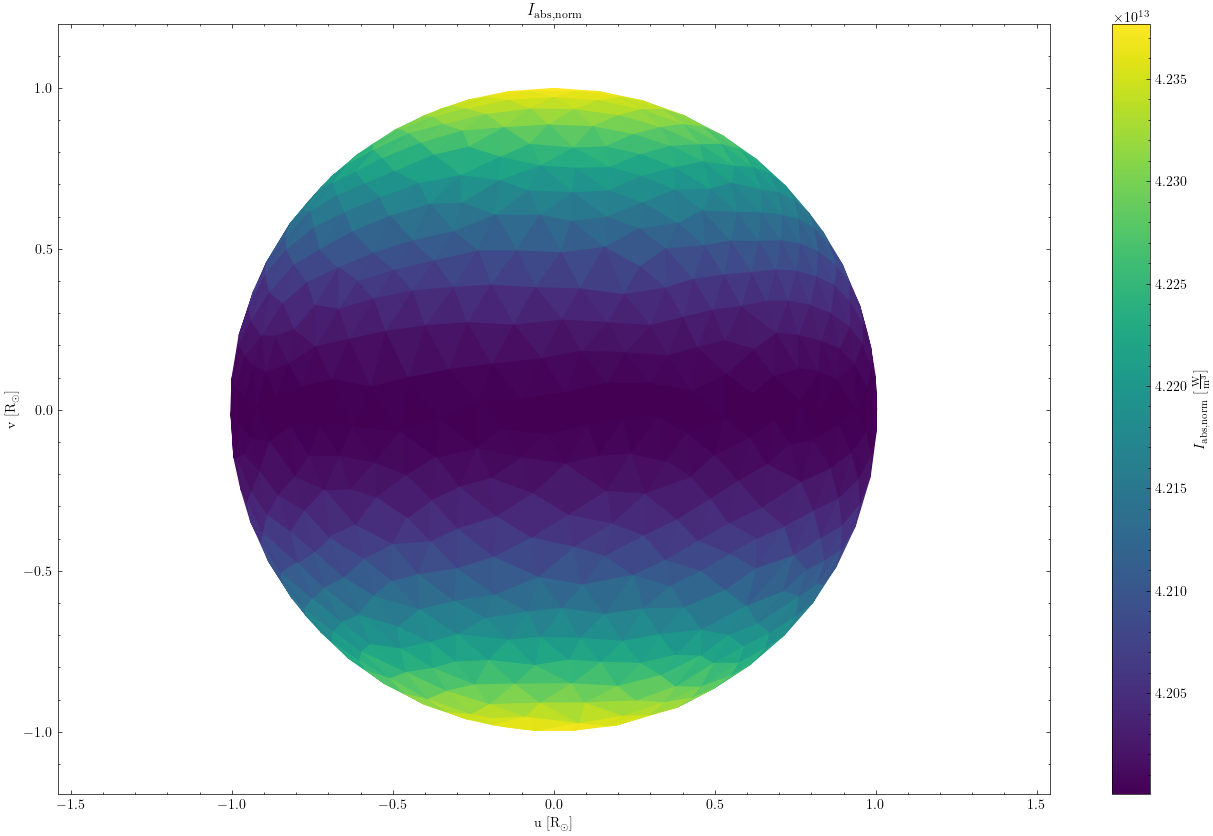
\includegraphics[scale=0.4]{Introduccion/Figures/Figura PHOEBE Malla Intensidad Normal.png}
	\caption{Intensidad absoluta de una estrella modelada utilizando PHOEBE,
	integrada en las longitudes de onda que abarca el pasa banda de
	\textit{Johnson:V}. La figura muestra la intensidad absoluta en la dirección
	del vector normal a los elementos superficiales. Se puede apreciar la
	distribución de la intensidad, la cual sigue el mismo comportamiento de la
	gravedad superficial que se muestra en la
	\reffigure{figuraMallaPhoebeTeffLogg}.}
	\label{figuraMallaPhoebeIntensidadNormal}
\end{figure}

Utilizando la intensidad monocromática definida en la
\refequation{ecuacionIntensidadMonocromatica} se usa para definir la
\textbf{distribución espectral de energía} (\textbf{SED} por sus siglas en
inglés), donde $\mathcal{S} \equiv \mathrm{d}I_{\lambda}/\mathrm{d}\lambda$. El
SED calculado depende tanto en las propiedades de la estrella como en el modelo
empleado para su atmósfera estelar; en el caso de un cuerpo negro, su SED
depende solo de su temperatura efectiva, mientras que modelos como
\autocite{kurucz_atlas_1970} requieren parámetros adicionales como la
metalicidad estelar y gravedad superficial. Sin embargo, en el modelo hacia
adelante de una estrella es de gran importancia determinar la intensidad en una
\textit{pasa banda}; esta es definida por una curva de transmisión, la cual
describe la cantidad de radiación incidente que traspasa el sistema óptico.
PHOEBE tiene varias pasa bandas disponibles, como por ejemplo la de
\textit{Johnson:V} vista en la \reffigure{figuraPhoebePasabandaJohnsonV}.
Utilizando la pasa banda elegida y el SED calculado se computa la intensidad de
la pasa banda con la siguiente ecuación:

\begin{eqfloat}
	\centering
	\begin{equation}
		I_{\textrm{pb}} = \int_{\lambda}{\mathcal{S}(\lambda) \mathcal{P}(\lambda)\textrm{d}\lambda}
	\end{equation}
	\blankcaption
	\label{ecuacionIntensidadPasabanda}
\end{eqfloat}

Donde $I_{\mathrm{pb}}$ como $\mathcal{S}$ son funciones que toman de parámetro
de entrada las propiedades termodinámicas de la estrella, incluyendo incluso
efectos extrínsecos al sistema como la extinción interestelar
\autocite{prsa_phoebe_increased_model_fidelity_mesh_2016}. La intensidad
$I_{\mathrm{pb}}$ definida en la \refequation{ecuacionIntensidadPasabanda} solo
es apropiada para simular un detector calibrado por flujo de estrellas
estándares; para medir la intensidad con respecto al número de fotones
detectados es necesario dividir $I_{\mathrm{pb}}$ entre la energía del fotón
incidente, definida como $E_{\lambda} = hc/\lambda$, e integrar:

\begin{eqfloat}
	\centering
	\begin{equation}
		I_{\textrm{pb}, \textrm{fot}} = \int_{\lambda}{\left(\frac{\mathcal{S}(\lambda) \mathcal{P}(\lambda)}{E_{\lambda}}\textrm{d}\lambda \right)} = \frac{1}{hc} \int_{\lambda}{\lambda \mathcal{S}(\lambda) \mathcal{P}(\lambda) \textrm{d}\lambda}
	\end{equation}
\end{eqfloat}

Por último, se integra $I_{\mathrm{pb}, \mathrm{fot}}$ o $I_{\mathrm{pb}}$\textemdash
dependiendo si se desea el flujo por cuentas de fotones o en energía\textemdash
a lo largo de la superficie estelar visible para obtener el flujo emitido por la
estrella en la pasa banda deseada, llegando como resultado a una curva de luz
sintética como en la \reffigure{figuraPhoebeObservablesSinteticos}, la cual
forma la base del análisis fotométrico de un sistema binario estelar.

\begin{figure}[!ht]
	\centering
	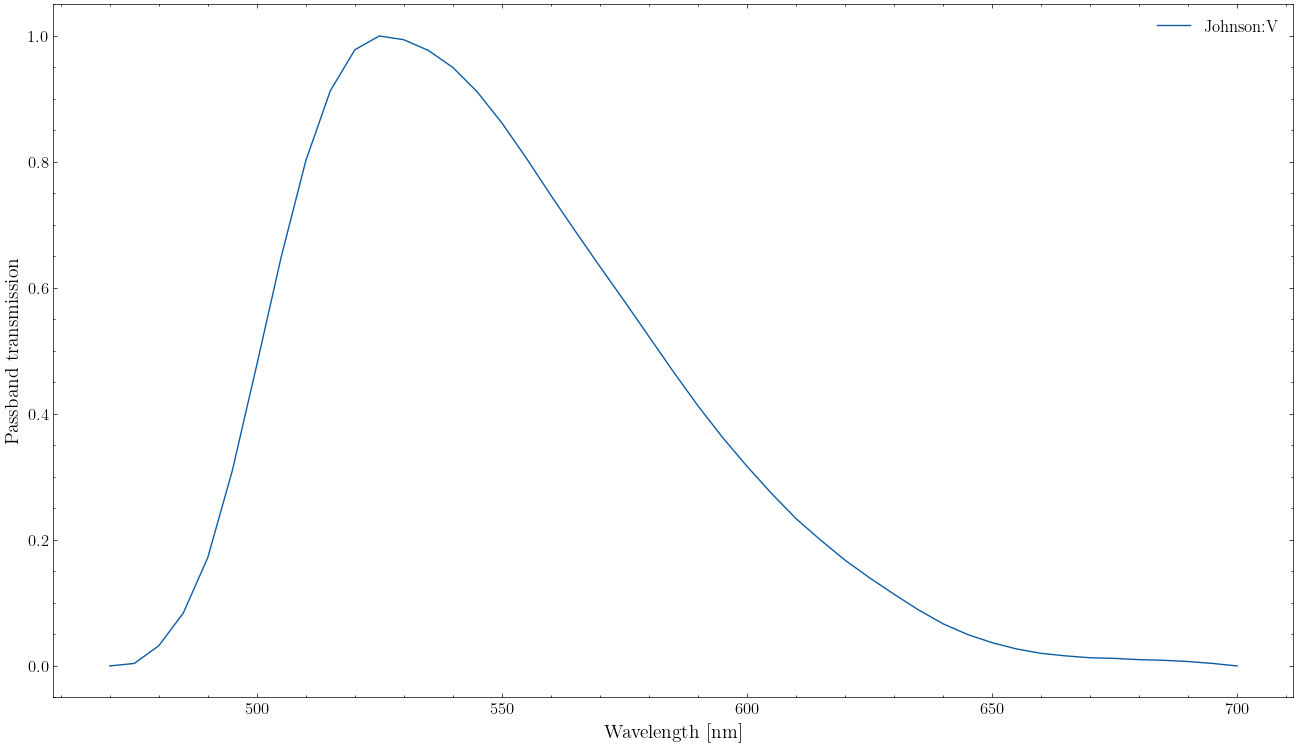
\includegraphics[scale=0.4]{Introduccion/Figures/Figura PHOEBE JohnsonV Pasabanda.png}
	\caption{Curva de transmisión en PHOEBE para la pasa banda \textit{Johnson:V}.}
	\label{figuraPhoebePasabandaJohnsonV}
\end{figure}

\section{El Problema Inverso}

El tener un modelo sofisticado de un sistema binario estelar nos ayuda a
entender los mecanismos responsables por su comportamiento, incluyendo como
afectan las diferentes combinaciones de parámetros estelares en las curvas
observables del sistema. Sin embargo, el propósito de modelos como PHOEBE o WD
yace en determinar los parámetros físicos que, una vez imputadas al modelo,
generan una curva observable sintética que se acopla a datos reales observados
del sistema. Esto en general se conoce como el \textbf{problema inverso}, y es
tanto una gran parte de este trabajo de tesis como el objetivo de varias
investigaciones en la literatura. Encontrar los parámetros que mejor ajustan un
modelo a datos observados es un proceso particular para cada objeto estudiado;
sin embargo, existe un proceso general que se sigue para llegar a una conclusión
cuyos errores y sesgos sean aceptables.

\subsection{Función de Calidad}

Para saber si un modelo es un buen ajusto a una curva observable de un sistema
es necesario definir una función que sirva para parametrizar el error entre el
modelo sintético y los datos reales. Para una curva observada, se calcula el
$\chi^2$, el cual se define como la siguiente expresión:

\begin{eqfloat}[!ht]
	\centering
	\begin{equation}
		\chi_{k}^2 = \sum_{i=1}^{N}{\left(\frac{y_{i,o} - y_{i,m}}{\sigma_{i}^2} + \ln{\sigma{i}^2}\right)}
	\end{equation}
	\blankcaption
	\label{ecuacionPhoebeChi2Curva}
\end{eqfloat}

Donde $y$ indica un punto en la curva del modelo, los subindices $o$ y $m$
refiriéndose a datos observacionales o del modelo sintético, respectivamente.
Cada punto del modelo se le atribuye un peso, la incertidumbre en el dato
observado $\sigma_{i,o}$, el cual se determina antes de ingresar los datos a
PHOEBE. En el caso de tener incertidumbres que han sido subestimadas se
introduce el termino $\sigma_{inf}$, donde al final se obtiene la incertidumbre
$\sigma_{i}$:

\begin{eqfloat}[!ht]
	\centering
	\begin{equation}
		\sigma_{i}^{2} = \sigma_{i,o}^{2} + y_{i,m}^{2} \exp{\left(2 \sigma_{inf}\right)}
	\end{equation}
\end{eqfloat}

En el caso de tener incertidumbres acertadas, $\sigma_{inf} = -\infty$, el cual
simplifica la previa ecuación a solo $\sigma_{i}^{2} = \sigma_{i,o}^{2}$.

Estos datos no necesariamente son mediciones fotométricas del sistema; pueden
ser velocidades radiales o intensidades de lineas espectrales. El subíndice $k$
denota la curva para la cual se está calculando el ajuste del modelo. Si se
tiene varias curvas observadas (por ejemplo, en diferentes bandas fotométricas)
el ajuste total del modelo se califica por la suma de los ajustes individuales a
cada curva observable:

\begin{eqfloat}[!ht]
	\centering
	\begin{equation}
		\chi^2 = \sum_{k}{\chi_{k}^{2}}
	\end{equation}
	\blankcaption
	\vspace{-0.4em}
	\label{ecuacionChi2}
\end{eqfloat}

El objetivo de un ajuste de un modelo a datos observacionales es encontrar los
parámetros físicos del sistema binario en cuestión que resultan en el $\chi^{2}$
más cercano a 0 posible. El valor obtenido de $\chi^2$ se parametriza en PHOEBE
normalizando por el número de observaciones hechas en todas las curvas de luz
combinadas $N_{\mathrm{tot}}$, resultando en el parámetro $\lambda$, el cual
indica un ajuste satisfactorio si $\lambda \approx 1$:

\begin{eqfloat}
	\centering
	\begin{equation}
		\lambda \coloneq \frac{\chi^2}{N_{\textrm{tot}}}
	\end{equation}
\end{eqfloat}

Sin embargo, el modelo descrito en la literatura, y que
usa PHOEBE, es altamente no-lineal; el espacio de parámetros posee una topología
compleja, el cual implica que existen más de una combinación de valores para los
parámetros del modelo que se ajustan a un mismo conjunto de curvas
observacionales, el cual se resalta en casos de degeneración de un modelo, donde
2 o más parámetros se ven correlacionados de tal manera que existen una cantidad
infinita de soluciones al problema. Para finalizar la descripción de PHOEBE con
respecto a este trabajo de tesis, se describe un proceso de ajuste de modelo a
un conjunto de curvas de luz fotométricas, utilizando herramientas dadas dentro
de PHOEBE, con la finalidad de llegar a la mejor combinación de parámetros
evitando caer lo más posible en trampas como mínimos locales en el espacio de
parámetros y modelos degenerados.

\subsection{Estimación Inicial de Parámetros}

La solución final para un sistema binario va a depender de manera significativa
de los valores iniciales de los cuales se parte las siguientes etapas del
ajuste. El proceso de estimar los valores iniciales es una combinación de
manipulación manual y herramientas diseñadas para un ajuste rápido a los datos
observacionales. Para utilizar estos estimadores es necesario primero encontrar
el periodo orbital del sistema, el cual comúnmente corresponde a la segunda
harmonica de la frecuencia dominante de un periodograma; los algoritmos
principales utilizados en la literatura son \textit{Lomb-Scargle}
\autocite{vanderplas_understanding_lomb_scargle_periodogram_2018} el cual ajusta
un modelo sinusoidal a una serie de tiempo (cuyas muestras no requieren haber
sido tomadas en intervalos regulares del tiempo) y \textit{Box Least Squares}
(abreviado como BLS) \autocite{kovacs_bls_periodogram_periodic_transits_2002},
un algoritmo diseñado para casos donde la señal de los eclipses es diminuto a
comparación con el flujo de base del sistema, por ejemplo los sistemas cuya
duración de eclipses estelares es mucho menor que el periodo orbital. Existen
varias implementaciones de periodogramas para su uso en el ámbito de la
astrofísica; ambos están disponibles dentro de PHOEBE en la forma de un
estimador:

% TODO: usar figure float o crear algo nuevo para solo bloques de código? pregunta a Dr.
\begin{figure}[!ht]
	\begin{lstlisting}[language=python, autogobble]
	periodogram_freqs = phoebe.linspace(0.001, MAX_FREQ, NUM_FREQS)
	b.add_solver('estimator.lc_periodogram', 
					solver='periodogram',
					algorithm='ls', # 'ls' corresponde a Lomb-Scargle, 'bls' a BLS
					sample_mode='manual',
					lc_datasets=['lc01', 'lc02'],
					sample_periods=periodogram_freqs)
	b.run_solver(solver='periodogram', solution='period_spectrum')
	\end{lstlisting}
	\caption{Ejemplo de cómo correr un periodograma de tipo
	Lomb-Scargle en un bundle de PHOEBE. Este caso en particular es para un
	modelo con 2 curvas de luz fotométricas distintas, que se ha determinado
	muestra un comportamiento sinusoidal. Dependiendo de la información
	antecedente disponible del objeto al estudiar se puede definir limites de
	manera manual del periodograma, por ejemplo si se sabe que es un sistema de
	corto periodo ($<$1 día). Los resultados del periodograma se pueden acceder en
	la solución \code{period\_spectrum}, donde se puede obtener el espectro de
	potencias completo.}
\end{figure}

Es posible correr un periodograma de manera automática o manual, dependiendo si
una malla de frecuencias es dada como entrada al periodograma. Una vez que se
obtenga el periodo orbital del sistema es posible determinar un punto de partida
de los parámetros del sistema, utilizando la curva de luz doblada en fase.
Dentro de PHOEBE existen 2 distintos métodos para esto: la estimación de
parámetros utilizando de manera directa la geometría de la curva, o haciendo uso
de \textbf{EBAI}.

\subsubsection{Geometría de la Curva de Luz}
Dada una curva de luz fotométrica en fase es posible estimar ciertos parámetros
del sistema analizando ciertas de sus características geométricas. Una vez que
se haya encontrado el periodo orbital del sistema\textemdash y por ende haber
obtenido la curva de luz en fase\textemdash es posible ajustar una función
analítica compuesta de 2 funciones Gaussianas, un término coseno, un término
constante, o cualquier combinación de estas que mejor se ajusten a los datos
observacionales, generando en total 7 modelos
\autocite{conroy_phoebe_v_framework_solving_inverse_problem_2020}. Utilizando un
ajuste de mínimos cuadrados a las curvas en fase, una vez estimado los tiempos
de los eclipses, se determina el mejor modelo usando un criterio. Del modelo
final se obtiene valores iniciales para tanto propiedades orbitales del
sistema\textemdash el tiempo de superconjunción primario $t_0$, la excentricidad
$e$, y el argumento de periastro $\omega_0$\textemdash como propiedades
relativas entre las estrellas componentes: la suma de radios normalizado al
semieje mayor de la órbita $(R_1 + R_2)/a_{\mathrm{orb}}$ (esto se nota en la
diferencia de anchura entre ambas jorobas de la curva de luz) y la razón de
temperaturas efectivas $T_{\mathrm{eff},2}/T_{\mathrm{eff},1}$ (el cual se puede
aproximar por la diferencia de profundidad entre el eclipse primario y
secundario). Este estimador solo es capaz de analizar sistemas separados, por lo
cual no se utilizó en este trabajo de tesis.

\subsubsection{EBAI - Eclipsing Binaries via Artificial Intelligence}
\textbf{EBAI} es una red neuronal artificial que hace uso de métodos de
aprendizaje automático como \textit{K-Nearest Neighbors} para mapear una curva
de luz observacional a parámetros físicos de un sistema binario estelar. El
algoritmo KNN ajusta una función a datos reales, permitiendo hacer una regresión
basado en los vecinos cercanos de un punto. Los detalles de KNN se encuentran en
\autocite{pedregosa_scikit-learn_2011}, el cual describe la implementación
dentro del paquete de Python \code{scikit-learn}. Una red neuronal es compuesta
de varias capas de procesamiento, donde cada capa está compuesta de unidades
individuales (o \quotes{neuronas}) que propagan valores de acuerdo a su función
de activación. Esta arquitectura es la que las permite \quotes{aprender}
relaciones en modelos no lineales como el de un sistema binario. Hasta el
momento (PHOEBE version $\leq$2.4.13) el estimador de EBAI es el único capaz de
estimar los parámetros de un sistema binario en contacto; un esquema de su
composición interna se puede ver en la \reffigure{figuraPhoebeEbaiAnnDiagrama}.

\begin{figure}[!ht]
	\centering
	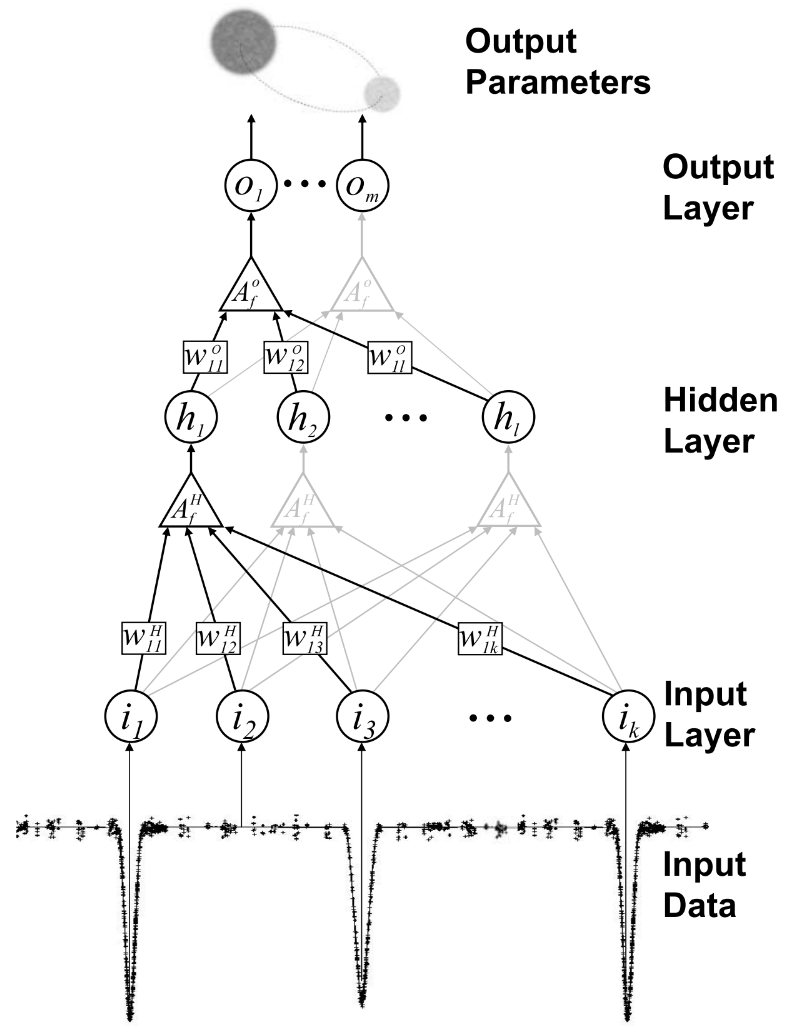
\includegraphics[scale=0.5]{Introduccion/Figures/Figura PHOEBE EBAI ANN Diagrama.png}
	\caption{Esquema de una red neuronal artificial (ANN por sus siglas en
	inglés). El objetivo de una red como EBAI es partir de datos de entrada como
	una curva de luz observada y obtener los parámetros del sistema que generen
	un modelo sintético que se aproxime a los datos. Figura obtenida de
	\autocite{prsa_phoebe_artificial_intelligence_approach_ebai_2008}.}
	\label{figuraPhoebeEbaiAnnDiagrama}
\end{figure}

Para sistemas binarios en contacto, el estimador EBAI puede determinar la razón
de masa $q$, la razón de temperaturas efectiva $T_2/T_1$, la inclinación orbital
$i$, y el factor de relleno $f$ del sistema; el estimador calcula un valor para
el tiempo de superconjunción $t_0$ del sistema binario, el cual es necesario
para obtener una curva de luz en fase cuyo eclipse primario yace en la fase
orbital 0. Dado un Bundle en PHOEBE, se puede generar una estimación inicial
corriendo el siguiente código:

\begin{figure}[!ht]
	\begin{lstlisting}[language=Python, autogobble]
	# b: phoebe.Bundle
	b.add_solver('estimator.ebai', solver='ebai_estimator', 
					ebai_method='knn', phase_bin=False, 
					lc_datasets=['lc01', 'lc02'])
	b.run_solver(solver='ebai_estimator', solution='ebai_init_estimates')
	b.adopt_solution(solution='ebai_init_estimates')
	\end{lstlisting}
	\caption{Código para correr un estimador EBAI para un sistema compuesto de 2
	curvas de luz fotométricas distintas, \code{lc01} y \code{lc02}. Para un
	sistema binario separado también existe la opción de correr el estimador con
	\code{ebai\_method='mlp'}, el cual usa una red neuronal propia de PHOEBE.}
\end{figure}

\subsection{Optimización de Parámetros}

Durante un ajuste de modelo es importante determinar si la combinación de
parámetros elegida es óptima dado una serie de datos observados. Esto se basa en
la función de costo definida en la \refequation{ecuacionChi2}; un ajuste
adecuado del modelo implica tener un valor de $\chi^2$ cercano a 0. PHOEBE
ofrece herramientas especializadas para encontrar la combinación de parámetros
que más se acerca a esta condición de manera sistemática. Estos son denominados
\textit{optimizadores}: algoritmos diseñados para explorar el espacio de
parámetros y llegar a un mínimo de la función de costo. Este trabajo de tesis
hizo uso de 2 optimizadores principales: \textbf{el simplex de Nelder-Mead} y
\textbf{correcciones diferenciales}.

\subsubsection{Simplex de Nelder-Mead}

Descrito por primera vez por \autocite{nelder_mead_simplex_1965}, el
\textbf{simplex de Nelder-Mead} (NMS por sus siglas en inglés) es un algoritmo
heurístico que explora el espacio de parámetros mediante un \textit{simplex}, un
politopo compuesto de varios vertices que representan distintos puntos en la
función que se busca optimizar. En el caso de PHOEBE, la función a optimizar es
$\chi^2$; para esto es necesario evaluar el ajuste en cada punto del simplex, lo
cual requiere calcular el modelo hacia adelante para cada punto de prueba. Esto
se demuestra con la siguiente modificación a la \refequation{ecuacionChi2}:

\begin{eqfloat}[!ht]
	\centering
	\begin{equation}
		\chi^2(\textbf{p}) = \sum_{i}{\frac{\left(F_{i}^{\textrm{obs}} - F^{\textrm{syn}}_i(\textbf{p})\right)^2}{\sigma_{i}^2}}
	\end{equation}
	\blankcaption
	\label{ecuacionChi2Params}
\end{eqfloat}

Donde $\mathbf{p}$ representa el vector de parámetros del modelo, como la
inclinación orbital, razón de masas, y cualquier otro incluido en el cálculo. El
método de NMS solo requiere evaluaciones de la función de costo en los puntos
del simplex; esto lo hace un método adecuado para optimizar funciones altamente
no-lineales a cambio de una baja eficiencia computacional 
dependiendo del número de vertices a evaluar. En total, la cantidad
de vertices empleados depende del número de dimensiones del modelo; en el caso
de optimizar $n$ parámetros del sistema binario, NMS utilizará $n+1$ vertices, o
combinaciones de parámetros. Con cada iteración, el método manipula el simplex
por medio de transformaciones geométricas, como lo muestra
\citetbooksection{phoebeScientificReference}{6.4}. En el ajuste de un sistema
binario eclipsante el método de NMS se utiliza para intentar llegar al mínimo
global de la función de costo, el cual el punto de parada es cuando haya
convergido la optimización (donde el simplex se podría considerar de un tamaño
geométrico despreciable), o cuando hayan pasado un cierto número de iteraciones,
en el caso que no haya sido completamente exitoso. Su uso se puede ver en la
\refcode{codigoOptimizadorNMS}. Para más información de la implementación y uso
del optimizador se puede hacer referencia a la documentación de
SciPy\footnote{\url{https://docs.scipy.org/doc/scipy/reference/optimize.minimize-neldermead.html}}

\begin{figure}[!ht]
	\centering
	\begin{lstlisting}[language=Python, autogobble]
	# b: phoebe.Bundle
	b.add_solver('optimizer.nelder_mead', solver='opt_nm', maxiter=50,
		fit_parameters=['teffratio', 'period@binary', 
			't0_supconj@binary', 'incl@binary', 'fillout_factor'])
	b.run_solver(solver='opt_nm', solution='opt_nm_solution')
	\end{lstlisting}
	\caption{Código para crear y ejecutar un optimizador utilizando el algoritmo
	NMS. Este código en particular busca encontrar la combinación de la razón de
	temperaturas, periodo orbital, el tiempo de superconjunción primario, la
	inclinación orbital, y el factor de relleno del sistema, como se puede ver
	por el argumento \code{fit\_parameters} del resolvedor (\textit{solver} por
	su categoría en inglés). Se especifica 50 como el máximo número de
	iteraciones que tiene permitido correr el optimizador en dado caso que no
	llegue a convergir a una solución; el criterio de convergencia se define por
	los argumentos \code{xatol} y \code{fatol} que definen una tolerancia de
	convergencia para los parámetros de entrada y la función de costo,
	respectivamente.}
	\label{codigoOptimizadorNMS}
\end{figure}

\subsubsection{Correcciones Diferenciales}

Una de las formas más directas de explorar el espacio de parámetros y llegar a
un valor optimo de la función de costo es por el método de \textbf{correcciones
diferenciales}. Este algoritmo trabaja evaluando derivadas parciales de la
función; estas son evaluadas por medio de diferencias finitas como se ve en la \refequation{ecuacionDiferenciasFinitas}.

\begin{eqfloat}[!ht]
	\centering
	\begin{equation}
		\frac{\partial f(p_1,...,p_k,...,p_n)}{\partial p_k} \rightarrow \frac{f(...p_k + \Delta p_k...) - f(...p_k...)}{\Delta p_k}
	\end{equation}
	\blankcaption
	\vspace{-0.4em}
	\label{ecuacionDiferenciasFinitas}
\end{eqfloat}

De esta manera PHOEBE explora el espacio alrededor de los valores actuales del
modelo para cada parámetro $p_k$; dado un valor de $\Delta p_k$ se calcula
$\chi^2$ en el punto actual del modelo y el paso propuesto, siguiendo el camino
que disminuya la función de costo. La técnica de correcciones diferenciales se
puede aplicar a más de un parámetro a la vez, evaluando la diferencia parcial
para cada parámetro a optimizar. Esta herramienta tiene mayor utilidad cuando el
modelo esté cerca del mínimo global, por ejemplo después obtener estimaciones
iniciales de los parámetros y utilizado un optimizador menos sensible a espacios
mínimos locales como NMS. Sin embargo, un algoritmo de correcciones
diferenciales puede divergir en modelos cuya discrepancia entre las curvas
sintéticas y curvas observadas es significativo. Es por esto que PHOEBE no
permite correr este optimizador por varias iteraciones de manera directa; esto
obliga al operador a analizar la solución propuesta por el algoritmo y decidir
si es una solución aceptable. Si es necesario ejecutar más iteraciones, el mismo
resolvedor es capaz de correr de nuevo, utilizando los valores adoptados de la
iteración pasada.

\subsection{Muestreo MCMC}

